\section{Failure Prediction}
\label{sec:approaches_failure_prediction}

\begin{figure}
\begin{subfigure}{\linewidth}
\centering
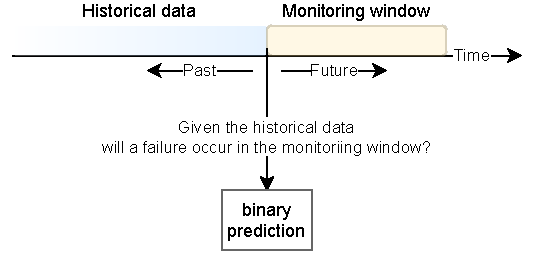
\includegraphics{approaches_failure_prediction_concept.pdf}
\caption{}
\end{subfigure}\\[1ex]
\begin{subfigure}{.5\linewidth}
\centering
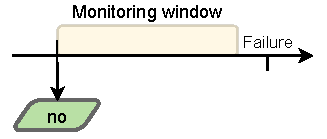
\includegraphics{approaches_failure_prediction_example_neg.pdf}
\caption{}
\end{subfigure}
\begin{subfigure}{.5\linewidth}
\centering
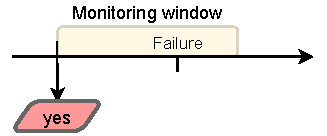
\includegraphics{approaches_failure_prediction_example_pos.pdf}
\caption{}
\end{subfigure}
\caption{Illustration of failure prediction:
        (a) general concept;
        (b) example of negative prediction, i.e. failure won't occur;
        (c) example of positive prediction, i.e. failure will occur.}
\label{fig:approaches_failure_prediction_illustration}
\end{figure}

Failure prediction is an approach where the goal is to make a binary prediction whether a failure will happen in near future --- in a monitoring window.
The concept of failure prediction is illustrated in the Figure 
\ref{fig:approaches_failure_prediction_illustration}.
Failure prediction approach is suitable in cases when there are available data about failures and when there are some patterns that precede the failure --- e.g. when an air compressor raises low pressure alarms before it fails.

\begin{figure}
    \includegraphics[width=.8\textwidth, keepaspectratio]{%
        approaches_failure_prediction_example_windows.pdf}
    \centering
    \caption{Illustration of monitoring, prediction and warning windows.}
    \label{fig:approaches_failure_prediction_example_windows}
\end{figure}

When predicting a failure, the domain problem might require the predictions to be made at least some time prior to the failure, e.g. the technicians have to be informed at least two days ahead in order to be able to schedule and perform the maintenance.
Therefore, a warning window might be specified which marks the minimal time prior to the failure in order for the prediction to be considered useful.
The time period of useful predictions is then called a prediction window and is defined as the time period between $t_F - M$ and $t_F - W$, where $t_F$ is a time stamp of the failure, $M$ is the size of the monitoring window and $W$ is the size of the warning window.
Figure \ref{fig:approaches_failure_prediction_example_windows} illustrates prediction and warning windows.

Failure prediction can be seen as a special case of fault detection where the prediction window are range-based faults.
However, failure prediction has some specifications in modeling and evaluation that differ from the range-based faults detection and thus we describe it as a special approach.

The concept of failure prediction is also used in many other domains such as healthcare, where heart failures are predicted, and it can also be found under name of early fault detection, early prediction of rare event, rare events prediction or rare events classification
\cite{ng2016early,weiss1998learning,ranjan2018dataset,choi2017using}.
In this thesis we will stick to the name failure prediction.

% TODO: add more literature that uses failure prediction and mention what other names they use for warning window etc.

\subsection{Data Specifications}

\begin{table}
	\centering
	\begin{tabular}{|c|c|cccc|c|}
    \hline
    subject id
    & time
    & \multicolumn{4}{|p{4cm}|}{\centering features}
    & failure event\\
    \hline
    subject 1 & 2020-01-01 &          0.1 &         0.05 & $\cdots$ &  34.1 & none \\
	subject 1 & 2020-01-02 &          0.3 &         0.12 & $\cdots$ &  34.2 & none \\
    $\vdots$ & $\vdots$ & $\vdots$ & $\vdots$ & $\ddots$ & $\vdots$ & $\vdots$ \\
    subject 1 & 2020-05-06 &          1.1 &         3.2 & $\cdots$ &  37.5 & none \\
    subject 1 & 2020-05-07 &          1.2 &         3.1 & $\cdots$ &  37.9 & failure A \\
    subject 1 & 2020-05-08 &          0.2 &         0.02 & $\cdots$ &  33.1 & none \\
    subject 1 & 2020-05-09 &          0.3 &         0.05 & $\cdots$ &  33.5 & none \\
    $\vdots$ & $\vdots$ & $\vdots$ & $\vdots$ & $\ddots$ & $\vdots$ & $\vdots$ \\
    subject 1 & 2020-07-29 &          2.5 &         0.21  & $\cdots$ &  35.9 & none \\
    subject 1 & 2020-07-30 &          2.2 &         0.2  & $\cdots$ &  36.1 & failure B \\
    $\vdots$ & $\vdots$ & $\vdots$ & $\vdots$ & $\ddots$ & $\vdots$ & $\vdots$ \\
	\end{tabular}
    \caption{A example of run-to-failure data set for failure prediction.}
    \label{tab:pdm_data_run_to_failure}
\end{table}

Data for training a failure prediction model must contain information about failures.
The data typically consist a condition monitoring data that are continuously collected during time and a failure log --- information when failures happened.
Such data are often called run-to-failure.
An example of run-to-failure data is illustrated in Table \ref{tab:pdm_data_run_to_failure}.
Moreover, it is necessary to have monitoring and warning windows.
However, it is good to note that the monitoring time does not have to be fixed.
Multiple models with different monitoring windows can be built and the choice of the final monitoring window can be made based on how the individual models perform.

\begin{figure}[H]
    \includegraphics[width=\textwidth, keepaspectratio]{%
        approaches_failure_prediction_modeling.pdf}
    \centering
    \caption{Diagram of modeling failure detection as time series
             point-based classification.}
    \label{fig:approaches_failure_prediction_modeling}
\end{figure}

\subsection{Modeling}

% \begin{figure}
%     \includegraphics[width=\textwidth, keepaspectratio]{%
%         approaches_failure_prediction_regression.png}
%     \centering
%     \caption{TODO}
%     \label{fig:approaches_failure_prediction_regression}
% \end{figure}

A failure prediction model can be built using a supervised classification algorithm where the samples in the training data are artificially labelled prior to the failure as positive.
Moreover, the predictions can be smoothed.
The whole modeling process is visualized in Figure
\ref{fig:approaches_failure_prediction_modeling} and described below.

\subsubsection{Artificial Labeling}

The classifier should learn to predict positive samples prior to failures.
Therefore, samples up to $M$ time steps prior to a failure are labeled as positive.
An example of artificial labeling with monitoring window of size 6 is illustrated in the upper part of Figure \ref{fig:approaches_failure_prediction_modeling}.

\subsubsection{Prediction}

The predictions are made point-wise by the trained classifier.
However, it might happen that there occur a single positive prediction among negative predictions due to a noise.
Therefore, the predictions can be smoothed using a rolling window and a positive prediction is assigned at time point $t$ when the ratio of positive predictions in the last $n$ predictions is higher  or equal than a given threshold.
We call the two parameters mentioned above a smoothing window and a smoothing threshold.
In case the classifier is capable of predicting probabilities of classes, the smoothing can be performed on the probabilities before the decision threshold is applied to avoid having two thresholds.

\subsection{Evaluation}
\label{sec:approaches_failure_prediction_evaluation}

In this section we describe how to evaluate the performance of a failure prediction model.
During evaluation we will aim to answer following questions:
\begin{itemize}
    \item What is the probability that the model will detect a failure?
    \item What is the probability that the model will make a false alarm? I.e. makes positive prediction but the failure won't occur in the monitoring window.
\end{itemize}
These questions are in \acrshort{ml} commonly answered by precision and recall metrics.
However, since we have more positive labels than failures due to artificial labeling, it is not straightforward how to use these metrics.
Below, we describe how to use classical precision and recall (described in Section \ref{sec:ml_evaluation}) and range-based precision and recall (described in Section \ref{sec:approaches_fault_detection_evaluation}) to evaluate a failure prediction model.
Next, we describe a modification of precision and recall, reduced precision and recall, introduced by Weiss et al. \cite{weiss1998learning}.
Finally, we propose new precision and recall metrics, a combination of the range-based metrics and the reduced metrics, that we call event-based precision and recall.

\subsubsection{Classical Precision and Recall}
\label{sec:approaches_failure_prediction_evaluation_classical_metrics}

This section describes how to use precision and recall using their standard definition (Section \ref{sec:ml_evaluation}) for failure prediction.

\begin{figure}
    \includegraphics[width=\textwidth, keepaspectratio]{%
        approaches_failure_prediction_evaluation.pdf}
    \centering
    \caption{Illustration of true labels and predictions in failure prediction.}
    \label{fig:approaches_failure_prediction_evaluation}
\end{figure}

As we use artificially created positive labels, we define following: 
\begin{enumerate}
    \item Actual positive samples are samples in the prediction windows, i.e. between $t_F - M$ and $t_F - W$.
    \item Actual negative samples are samples before $t_F - M$.
    \item Samples in the warning window, i.e. between $t_F - W$ and $t_F$, are not omitted from evaluation as they do not represent useful predictions.
\end{enumerate}

Figure \ref{fig:approaches_failure_prediction_evaluation} illustrates what time points are considered as positive and negative and which predictions are considered as \acrshort{tp}, \acrshort{tn}, \acrshort{fp} and \acrshort{fn}.
Recall and precision metrics are then used by their standard definition as:
\begin{align*}
    \text{recall} &= \frac{\text{TP}}{\text{P}},\\
    \text{precision} &= \frac{\text{TP}}{\text{TP} + \text{FP}}.
\end{align*}

\begin{figure}[hbt!]
    \includegraphics[width=.9\textwidth, keepaspectratio]{%
        approaches_failure_prediction_evaluation_recall_con.pdf}
    \centering
    \caption{Different predictions for the same data having the same recall score:
             (\textbf{left}) all of the three failures predicted
             (\textbf{right}) only one failure predicted.}
    \label{fig:approaches_failure_prediction_evaluation_recall_con}
\end{figure}

\begin{figure}[hbt!]
    \includegraphics[width=.75\textwidth, keepaspectratio]{%
        approaches_failure_prediction_evaluation_precision_con.pdf}
    \centering
    \caption{Different positions of two FPs having different severity:
             (\textbf{top}) far from each other
             --- such FPs can be considered as independent;
             (\textbf{middle}) close to each other
             --- the second FP is less serious and the two FPs can be almost
             considered as one;
             (\textbf{bottom}) close to each other and close to the monitoring period
             --- probably not so serious FPs as it might happen that the failure
             was predicted a bit sooner than at $t_F - M$.}
    \label{fig:approaches_failure_prediction_evaluation_precision_con}
\end{figure}

The classical metrics have two major issues:
\begin{itemize}
    \item Recall doesn't reflect how many failures were predicted.
    Figure \ref{fig:approaches_failure_prediction_evaluation_recall_con} shows examples of two models whose predictions have same recall score but they successfully predicted different number of failures.
    \item Precision doesn't reflect how close FPs are to each other.
    Figure \ref{fig:approaches_failure_prediction_evaluation_precision_con} shows examples of three series all having two \acrshort{fp}s but possibly having different importance in practice, e.g. two consecutive FPs may be treated as one FP whereas two FPs far from each other should count as two FPs.
\end{itemize}
Below, we describe three other types of precision and recall metrics that might mitigate these issues.

\subsubsection{Range-based Precision and Recall}

Failure prediction can be evaluated using range-based precision and recall as described in Section \ref{sec:approaches_fault_detection_evaluation} by taking the prediction windows as real fault (anomaly) ranges and consecutive positive predictions as predicted ranges.
Setting a non-zero existence weight $\alpha$ to the detection score of the range-based metrics solves the first issue mentioned above --- recall not reflecting how many failures were predicted.

\subsubsection{Reduced Precision and Recall}

Weiss et al. introduced in 1998 evaluation metrics called reduced precision and recall for prediction of rare events in time series \cite{weiss1998learning} which is a problem identical to failure prediction.
The main idea of the reduced metrics is to use the number of events (failures) instead of positive samples, use the number of predicted events instead of TP and use discounted FP instead of FP.

\paragraph{P $\rightarrow$ TotalEvents}
The total number of events (failures) is used instead of positive samples.
This means that for every prediction window consisting of $M - W$ samples there is one even, i.e. total number of events is equal to dividing the number of positives by the size of a prediction window.

\begin{figure}
    \centering
    \begin{subfigure}{.45\textwidth}
        \centering
        \includegraphics[width=.7\linewidth]{%
            approaches_failure_prediction_evaluation_failure_predicted.pdf}
        \caption{Failures predicted}
      \label{fig:approaches_failure_prediction_evaluation_failure_predicted}
    \end{subfigure}%
    \begin{subfigure}{.45\textwidth}
        \centering
        \includegraphics[width=.7\linewidth]{%
            approaches_failure_prediction_evaluation_failure_not_predicted.pdf}
        \caption{Failures not predicted}
        \label{fig:approaches_failure_prediction_evaluation_failure_not_predicted}
    \end{subfigure}
    \caption{Illustrations of events (failures) being and not being predicted}
\end{figure}

\paragraph{TP $\rightarrow$ EventsPredicted}
The true positives are replaced by the number of predicted events.
The event is considered as predicted when there is at least one positive prediction in its prediction window, i.e. at least $W$ and at most $M$ time steps prior to the event.
Figures \ref{fig:approaches_failure_prediction_evaluation_failure_predicted} and \ref{fig:approaches_failure_prediction_evaluation_failure_not_predicted} illustrate examples of events being predicted and not being predicted, respectively.

\begin{figure}
    \includegraphics[width=.75\textwidth, keepaspectratio]{%
        approaches_failure_prediction_evaluation_discounted_fp.pdf}
    \centering
    \caption{Illustration of calculating DiscountedFP.}
    \label{fig:approaches_failure_prediction_evaluation_discounted_fp}
\end{figure}

\paragraph{FP $\rightarrow$ DiscountedFP}
Every positive prediction has a meaning that an event (failure) will happen in the monitoring window.
If there are two consecutive positive predictions, the latter prediction can be considered as having lesser severity as the two consecutive predictions can be regarded as one false alarm.
Therefore, Weiss et al. define calculate as the number of complete, non-overlapping, monitoring windows associated with a false positive \cite{weiss1998learning}.
For example when having monitoring window of size 10, two consecutive false positives will produce a discounted FP of 1.1, i.e. 1 for the first prediction plus 0.1 for the second.
If the there is a false positive at time point $t$ and a false positive at time point $t + 5$, then the discounted FP for these two false positives will be equal 1.5.
Figure \ref{fig:approaches_failure_prediction_evaluation_discounted_fp} illustrates how discounted FP is calculated in three different scenarios.

The reduced precision and recall metrics are then defined as:
\begin{align*}
    \text{reduced recall} &= \frac{\text{EventsPredicted}}{\text{TotalEvents}},\\
    \text{reduced precision} &=
    \frac{\text{EventsPredicted}}
    {\text{EventsPredicted} + \text{DiscountedFP}}.
\end{align*}

Reduced recall is then identical to range-based precision when setting $\alpha = 1$, i.e. taking into account only the existence of a positive prediction in the prediction window.

\subsubsection{Event-based Precision and Recall}

Above, we described how range-based and reduced metrics can be used for failure prediction.
In this section, we propose a combination of the range-based and the reduced metrics.
The combination consists in taking the reduced metrics replacing the number of events predicted by a sum of detection scores from the range-based metrics.
We call such metrics event-based precision and recall and define it as follows:
\begin{align*}
    \text{event-based recall} &= \frac{\sum\text{DetectionScore}}{\text{Events}},\\
    \text{event-based precision} &=
    \frac{\sum\text{DetectionScore}}
    {\sum\text{DetectionScore} + \text{DiscountedFP}}.
\end{align*}
where $\sum\text{DetectionScore}$ is a sum of detection scores for all the prediction windows.